\documentclass[12pt,dvipdfmx]{beamer}
\usepackage{graphicx}
\DeclareGraphicsExtensions{.pdf}
\DeclareGraphicsExtensions{.eps}
\graphicspath{{out/tex/svg/}{out/pdf/svg/}}
\usepackage{listings}
\usepackage{fancybox}
\usepackage{hyperref}
\usepackage{color}

\newcommand{\plusequal}{\mbox{\tt\ += }}
\newcommand{\minusequal}{\mbox{\tt\ -= }}
\newcommand{\divequal}{\mbox{\tt\ /= }}
\newcommand{\plusplus}{\mbox{\tt\ ++ }}



%% OpenMP section numbers
\newcommand{\sectionompparallel}{2.5}
\newcommand{\sectionompdeterminenumthreads}{2.5.1}
\newcommand{\sectionompfor}{2.7.1}
\newcommand{\sectionompdataenv}{2.14}
\newcommand{\sectionompgetnumthreads}{3.2.2}
\newcommand{\sectionompgetmaxthreads}{3.2.3}
\newcommand{\sectionompgetthreadnum}{3.2.4}


%%%%%%%%%%%%%%%%%%%%%%%%%%%
%%% themes
%%%%%%%%%%%%%%%%%%%%%%%%%%%
%\usetheme{Szeged} 
\usetheme{Madrid}

%% no navigation bar
% default boxes Bergen Boadilla Madrid Pittsburgh Rochester
%% tree-like navigation bar
% Antibes JuanLesPins Montpellier
%% toc sidebar
% Berkeley PaloAlto Goettingen Marburg Hannover Berlin Ilmenau Dresden Darmstadt Frankfurt Singapore Szeged
%% Section and Subsection Tables
% Copenhagen Luebeck Malmoe Warsaw

%%%%%%%%%%%%%%%%%%%%%%%%%%%
%%% innerthemes
%%%%%%%%%%%%%%%%%%%%%%%%%%%
% \useinnertheme{circles}	% default circles rectangles rounded inmargin

%%%%%%%%%%%%%%%%%%%%%%%%%%%
%%% outerthemes
%%%%%%%%%%%%%%%%%%%%%%%%%%%
% outertheme
% \useoutertheme{default}	% default infolines miniframes smoothbars sidebar sprit shadow tree smoothtree


%%%%%%%%%%%%%%%%%%%%%%%%%%%
%%% colorthemes
%%%%%%%%%%%%%%%%%%%%%%%%%%%
\usecolortheme{seahorse}
%% special purpose
% default structure sidebartab 
%% complete 
% albatross beetle crane dove fly seagull 
%% inner
% lily orchid rose
%% outer
% whale seahorse dolphin

%%%%%%%%%%%%%%%%%%%%%%%%%%%
%%% fontthemes
%%%%%%%%%%%%%%%%%%%%%%%%%%%
\usefonttheme{serif}  
% default professionalfonts serif structurebold structureitalicserif structuresmallcapsserif

%%%%%%%%%%%%%%%%%%%%%%%%%%%
%%% generally useful beamer settings
%%%%%%%%%%%%%%%%%%%%%%%%%%%
% 
\AtBeginDvi{\special{pdf:tounicode EUC-UCS2}}
% do not show navigation
\setbeamertemplate{navigation symbols}{}
% show page numbers
\setbeamertemplate{footline}[frame number]


%%%%%%%%%%%%%%%%%%%%%%%%%%%
%%% define some colors for convenience
%%%%%%%%%%%%%%%%%%%%%%%%%%%

%\newcommand{\mido}[1]{{\color{green}#1}}
\newcommand{\mido}[1]{{\color{green}#1}}
\newcommand{\mura}[1]{{\color{purple}#1}}
\newcommand{\ore}[1]{{\color{orange}#1}}
\newcommand{\ao}[1]{{\color{blue}#1}}
\newcommand{\aka}[1]{{\color{red}#1}}

\setbeamercolor{ex}{bg=cyan!20!white}

%%%%%%%%%%%%%%%%%%%%%%%%%%%
%%% how to typset code
%%%%%%%%%%%%%%%%%%%%%%%%%%%

\lstset{language = C,
numbers = left,
numberstyle = {\tiny \emph},
numbersep = 10pt,
breaklines = true,
breakindent = 40pt,
frame = tlRB,
frameround = ffft,
framesep = 3pt,
rulesep = 1pt,
rulecolor = {\color{blue}},
rulesepcolor = {\color{blue}},
flexiblecolumns = true,
keepspaces = true,
basicstyle = \ttfamily\scriptsize,
identifierstyle = ,
commentstyle = \it\scriptsize,
stringstyle = ,
showstringspaces = false,
tabsize = 4,
escapechar=\@,
}

\title{Parallel and Distributed Programming \\ Introduction}
\institute{}
\author{Kenjiro Taura}
\date{}

\AtBeginSection[] % Do nothing for \section*
{
\begin{frame}
\frametitle{Contents}
\tableofcontents[currentsection,currentsubsection]
\end{frame}
}

\AtBeginSubsection[] % Do nothing for \section*
{
\begin{frame}
\frametitle{Contents}
\tableofcontents[currentsection,currentsubsection]
\end{frame}
}

\begin{document}
\maketitle

%%%%%%%%%%%%%%%%%%%%%%%%%%%%%%%%%% 
\begin{frame}
\frametitle{Contents}
\tableofcontents
\end{frame}

%=================================
\section{Why Parallel Programming?}
%=================================

%%%%%%%%%%%%%%%%% 
\begin{frame}
\frametitle{Why parallel?}
\begin{itemize}
\item<1-> frequencies no longer increase \ao{(end of Dennard scaling)}
\item<2-> techniques to increase performance 
  (Instruction-Level Parallelism, or ILP) of serial programs are increasingly
  difficult to pay off \ao{(Pollack's law)}
\item<3-> multicore, manycore, and GPUs are in part response to it
  \begin{center}
  \item \ao{\textit{have more transistors? $\Rightarrow$ have more cores}}
  \end{center}
\end{itemize}

\begin{center}
  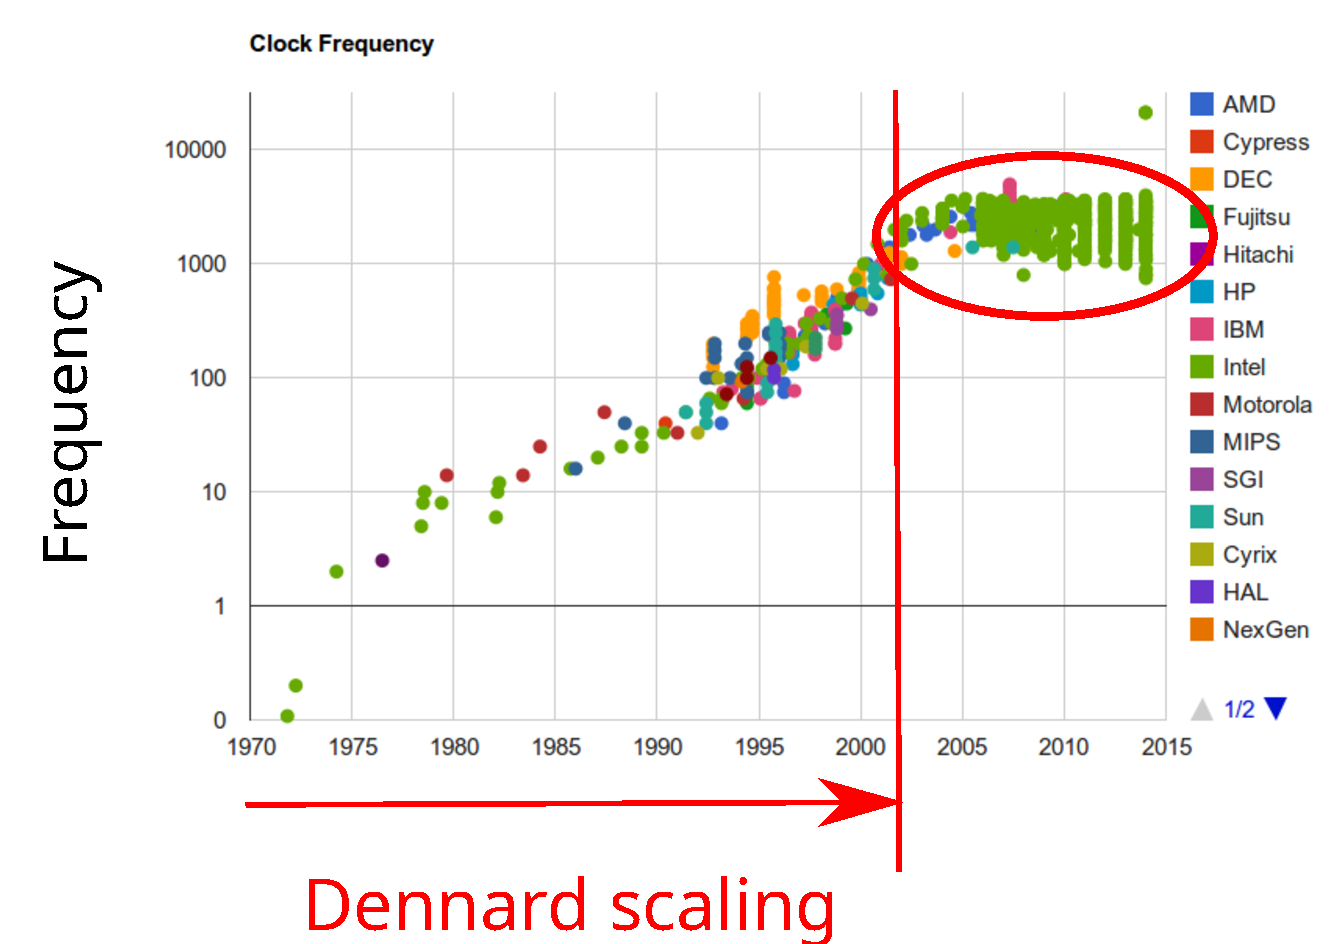
\includegraphics[width=0.45\textwidth]{out/pdf/svg/frequency.pdf}
    
  source: \url{http://cpudb.stanford.edu/}
\end{center}
\end{frame}

%%%%%%%%%%%%%%%%% 
\begin{frame}
\frametitle{There are no serial machines any more}
\begin{itemize}
\item virtually all CPUs are now \ao{\textit{multicore}}
\item high performance accelerators (GPUs and Xeon Phi) run at
  even low frequencies and have many more cores \ao{\textit{(manycore)}}
\end{itemize}
\end{frame}

%%%%%%%%%%%%%%%%% 
\begin{frame}
\frametitle{Processors for supercomputers are ordinary, perhaps even more so}
  \begin{center}
    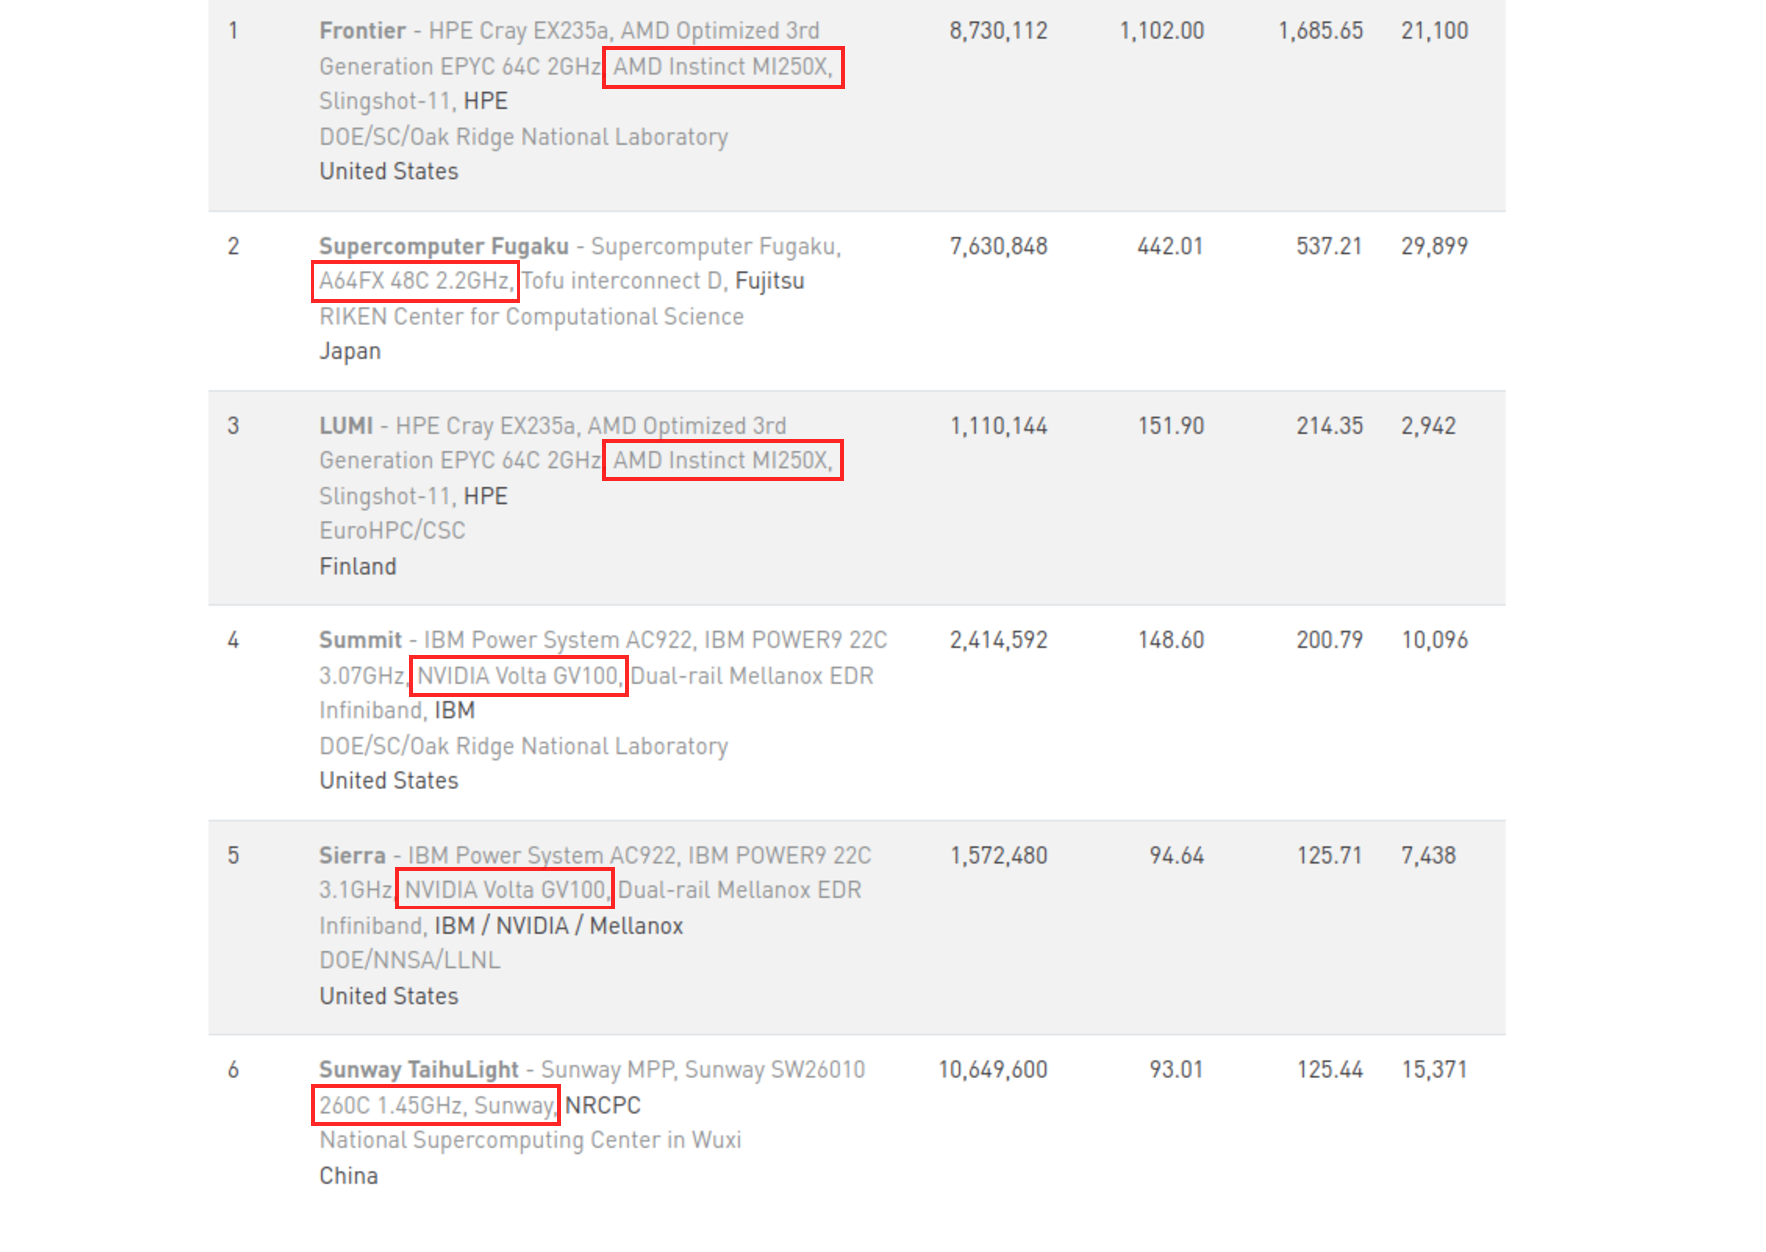
\includegraphics[width=0.7\textwidth]{out/pdf/svg/top500_2022_june.pdf}

    \url{https://www.top500.org/lists/top500/2022/06/}
  \end{center}
\end{frame}

\iffalse
%%%%%%%%%%%%%%%%% 
\begin{frame}
\frametitle{More in the list}
  \begin{center}
    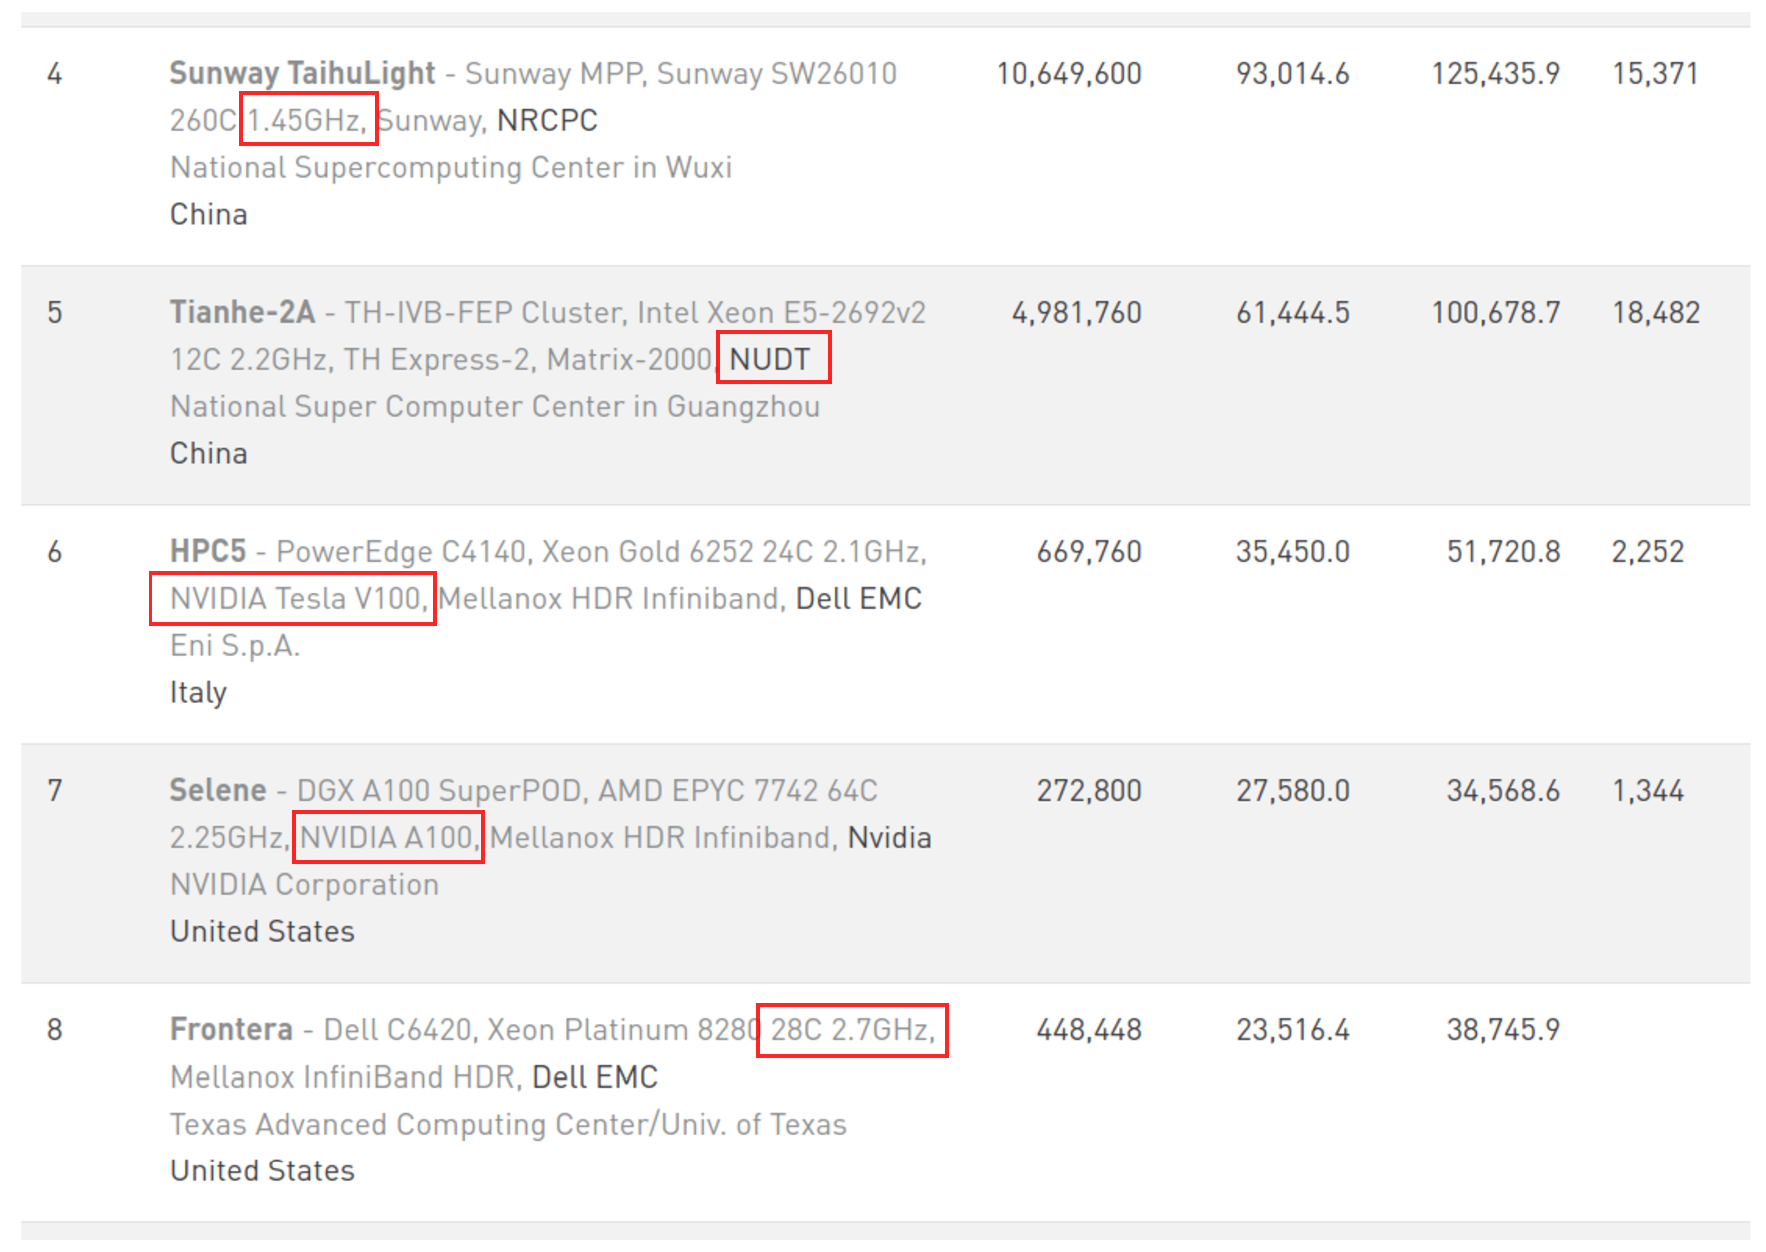
\includegraphics[width=0.6\textwidth]{out/pdf/svg/top500_2020_june_2.pdf}

    \url{https://www.top500.org/}
  \end{center}
  \begin{columns}
    \begin{column}{0.5\textwidth}
      {\footnotesize
        \begin{itemize}
        \item Fugaku ($\approx$ 2.2GHz)
        \item NVIDIA GPU ($\approx$ 1 - 1.5GHz)
        \end{itemize}}
    \end{column}
    \begin{column}{0.5\textwidth}
      {\footnotesize
        \begin{itemize}
        \item Sunway ($\approx$ 1.45GHz)
        \item Intel CPUs running at $\approx$ 2.0GHz
        \end{itemize}}
    \end{column}
  \end{columns}
\end{frame}
\fi

%%%%%%%%%%%%%%%%% 
\begin{frame}
\frametitle{Implication to software}
\begin{itemize}
\item<1-> existing serial SWs do not get (dramatically) faster on new CPUs
\item<2-> just writing it in C/C++ goes nowhere close to machine's potential performance,
  unless you know how to exploit parallelism of the machine
\item<3-> you need to understand
  \begin{itemize}
  \item does it use multiple cores (and how the work is distributed)?
  \item does it use SIMD instructions?
  \item does it have good instruction level parallelism?
  \end{itemize}
\end{itemize}
\end{frame}

%%%%%%%%%%%%%%%%% 
\begin{frame}[fragile]
\frametitle{Example: matrix multiply}

\begin{itemize}
\item []
  \begin{itemize}
  \item how much can we improve this on a single machine?
  \end{itemize}

\begin{lstlisting}
void gemm(long M, long N, long K,
          float A[M][K], float B[K][N], float C[M][N]) {
  long i, j, k;
  for (i = 0; i < M; i++)
    for (j = 0; j < N; j++)
      for (k = 0; k < K; k++)
        C[i][j] += A[i][k] * B[k][j];
}
\end{lstlisting}

% \item<2-> []
% \begin{lstlisting}
% $ make
% gcc -O3 -o simple_mm mm.c
% gcc -O3 -DUSE_BLAS -o blas_mm mm.c -lopenblas
% \end{lstlisting} %$

\iffalse
\item<2-> []
\begin{lstlisting}
$ ./simple_mm 
C[1200][1200] = 3011.114014
 in 56.382360 sec
 @\ao{\texttt{2.451831 GFLOPS}}@
\end{lstlisting} %$

\item<3-> []
\begin{lstlisting}
$ ./opt_mm 
C[1200][1200] = 3011.108154
 in 1.302980 sec
 @\ao{\texttt{106.095263 GFLOPS}}@
\end{lstlisting} %$
\fi
\end{itemize}

\end{frame}


%=================================
\section{What Parallel Machines Look Like, and Where Performance Come From?}
%=================================

%%%%%%%%%%%%%%%%% 
\begin{frame}
\frametitle{What a single parallel machine (node) looks like}
\begin{columns}
\begin{column}{0.4\textwidth}
\begin{center}
\only<1>{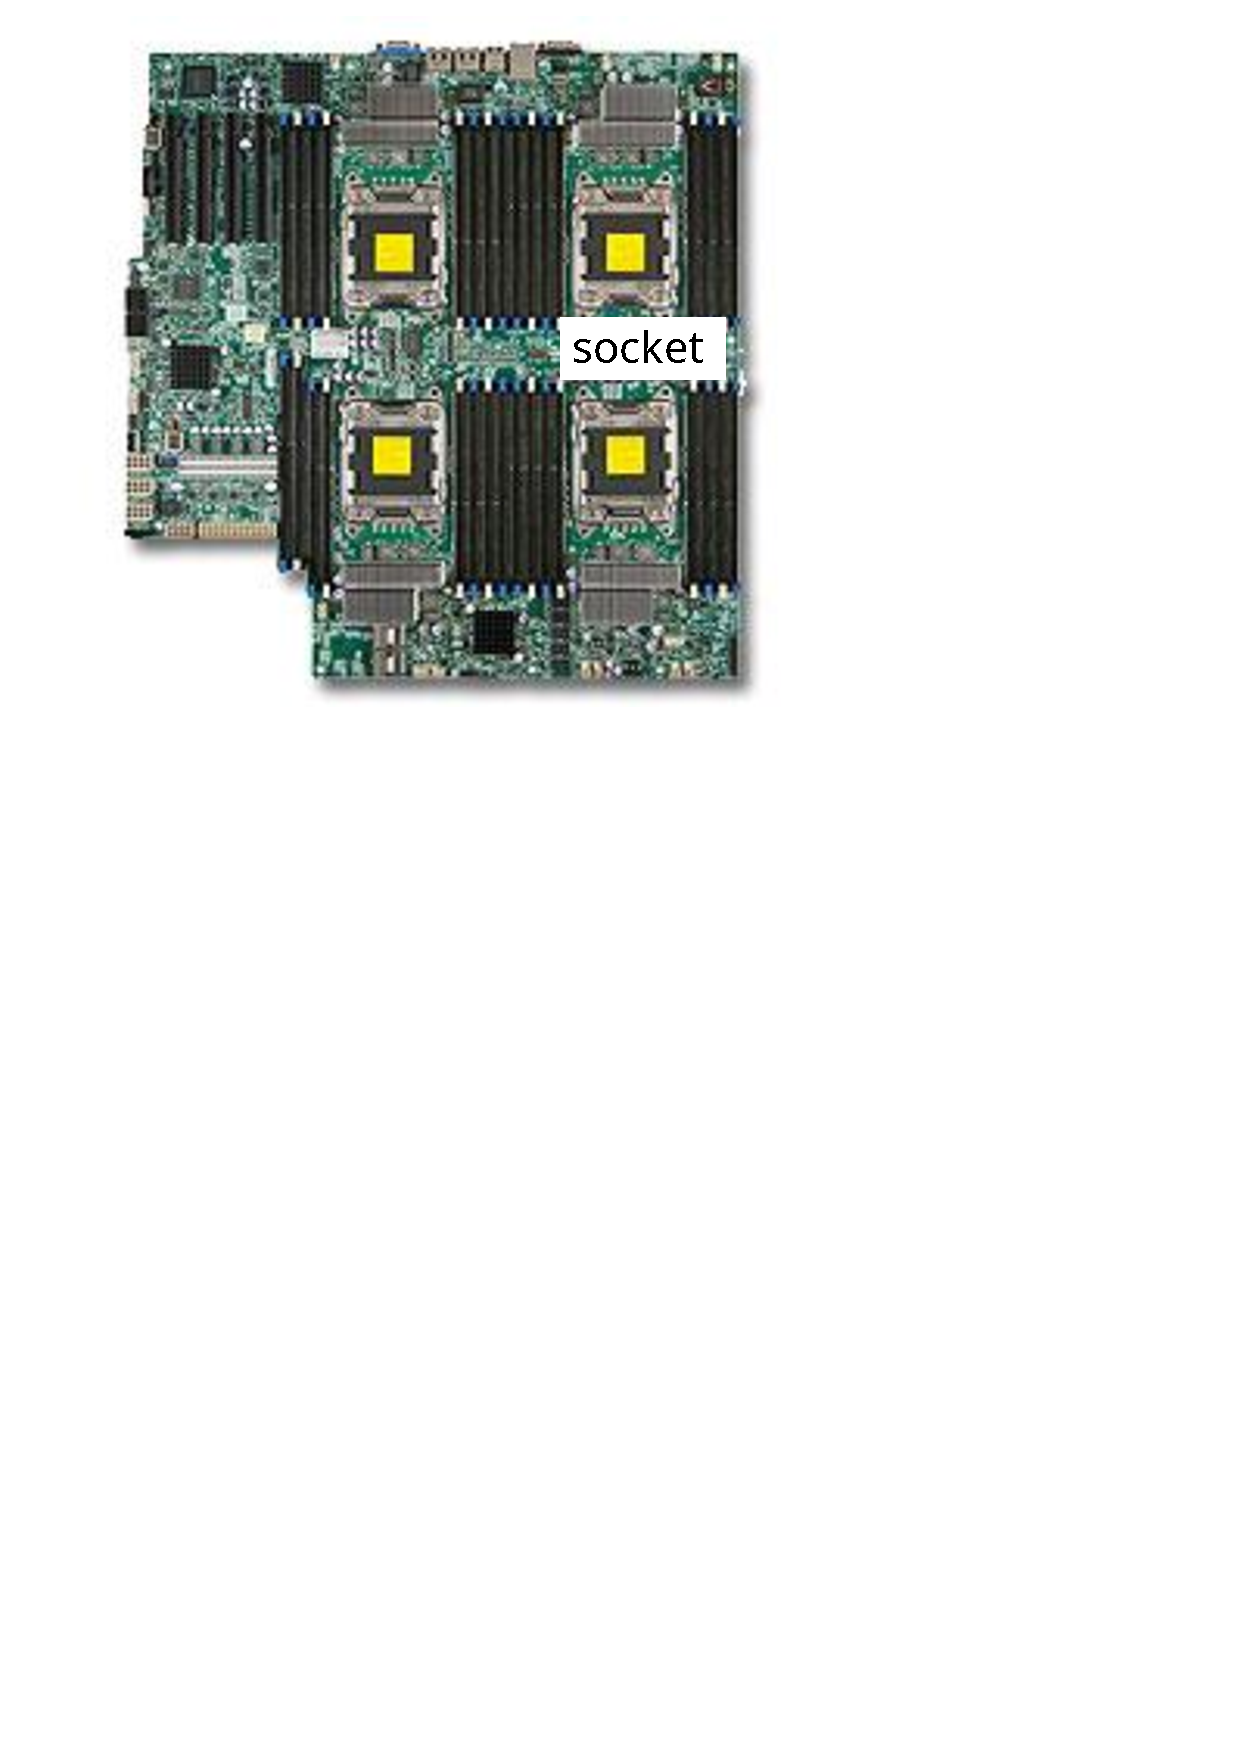
\includegraphics[width=\textwidth]{out/pdf/svg/quad_mother_board_0.pdf}}%
\only<2>{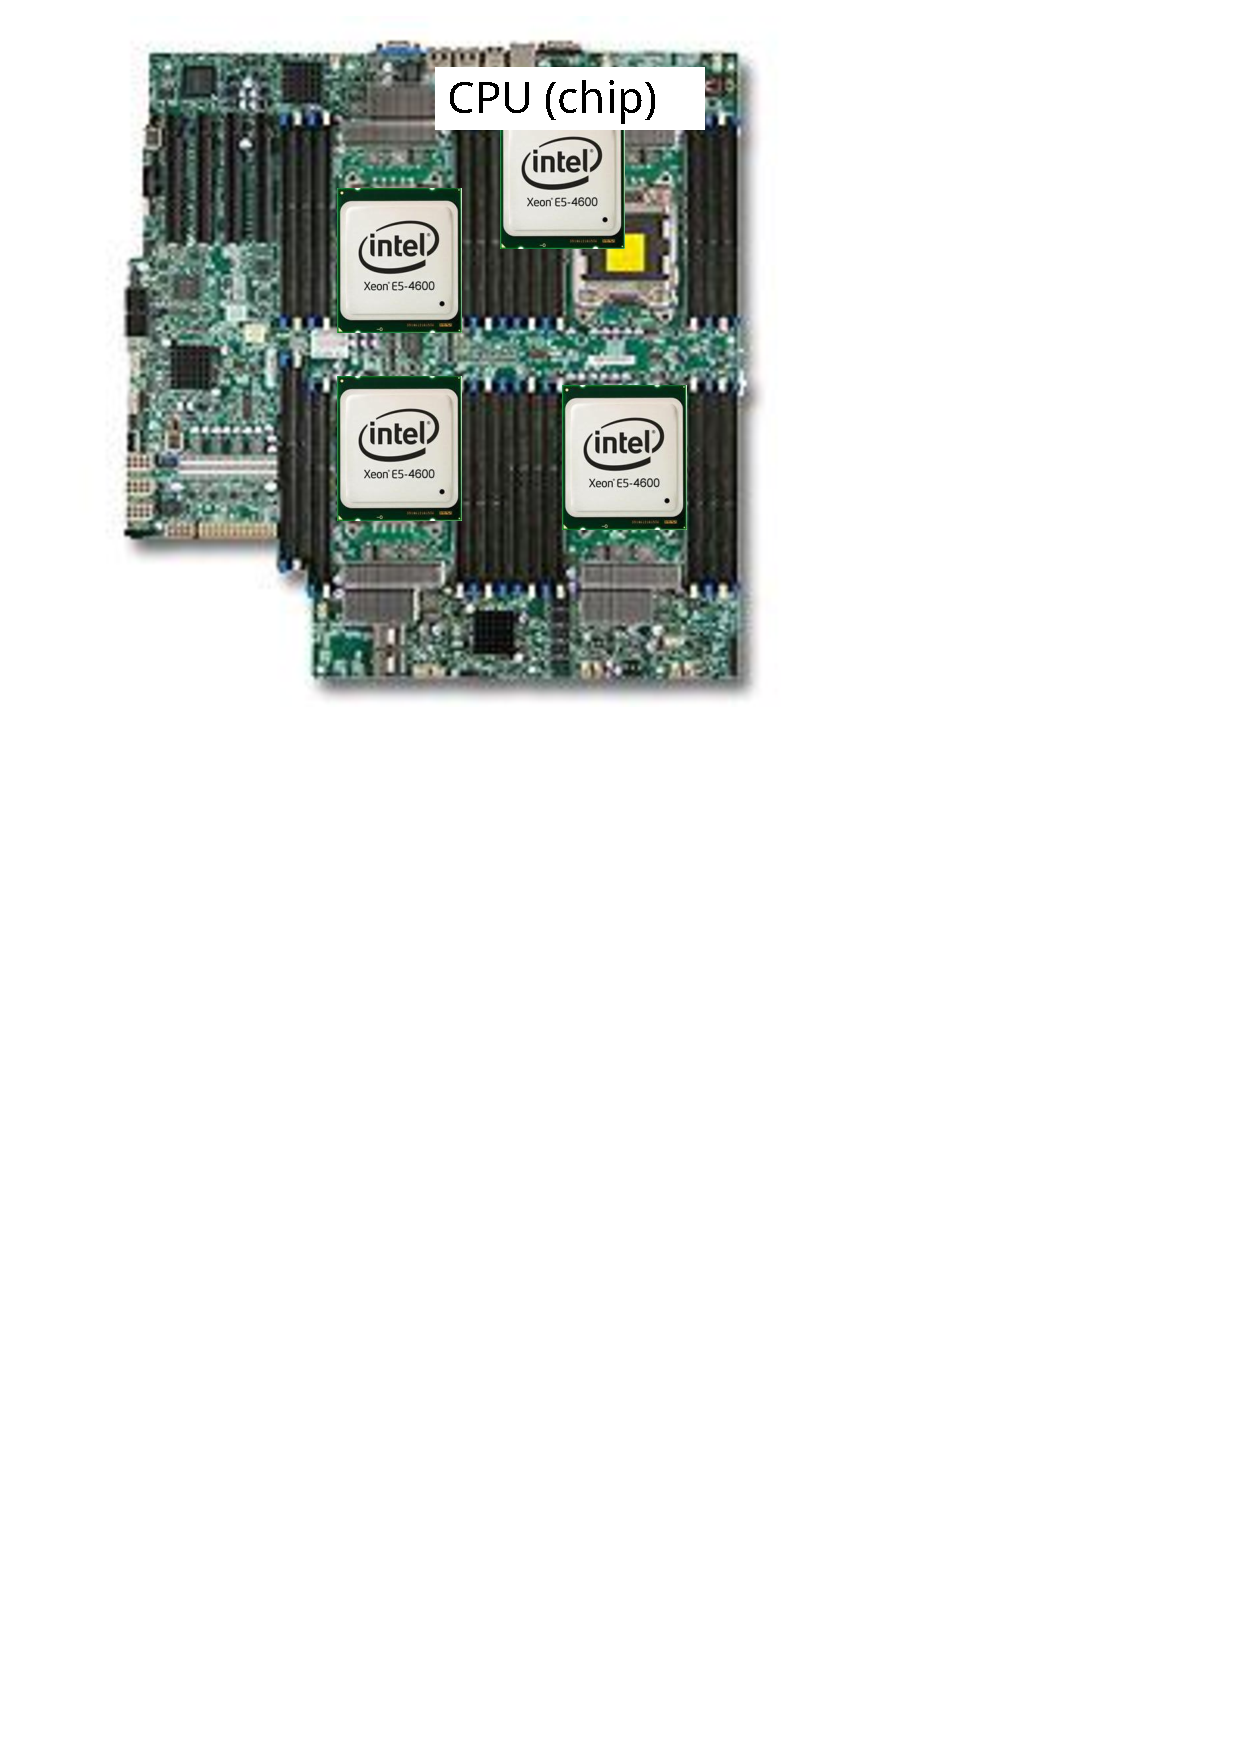
\includegraphics[width=\textwidth]{out/pdf/svg/quad_mother_board_1.pdf}}%
\only<3>{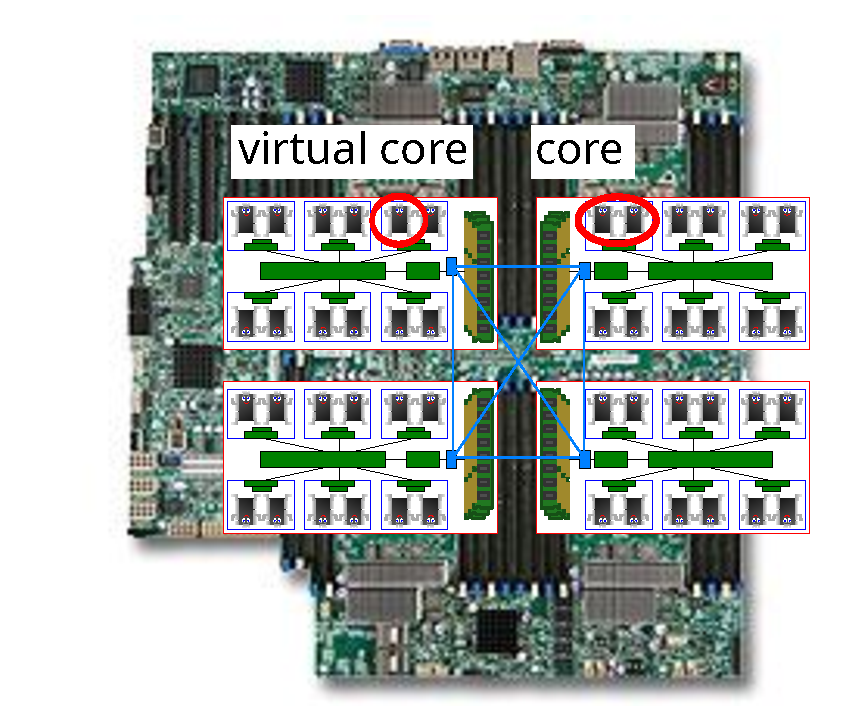
\includegraphics[width=\textwidth]{out/pdf/svg/quad_mother_board_diagram.pdf}}
\end{center}
\end{column}
\begin{column}{0.6\textwidth}
\begin{center}
  % 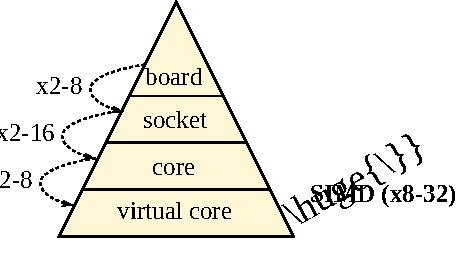
\includegraphics[width=\textwidth]{out/pdf/svg/hierarchy.pdf}
\def\svgwidth{0.7\textwidth}
\input{out/tex/svg/hierarchy.pdf_tex}
\end{center}
\end{column}
\end{columns}

\begin{itemize}
\item SIMD : Single Instruction Multiple Data
\item a single SIMD register holds many values
\item a single instruction applies the same operation (e.g., add, multiply, etc.)
  on all data in a SIMD register
\item a single core can execute multiple instructions in each cycle (ILP)
\end{itemize}
\end{frame}

%%%%%%%%%%%%%%%%% 
\begin{frame}
\frametitle{What a machine looks like}
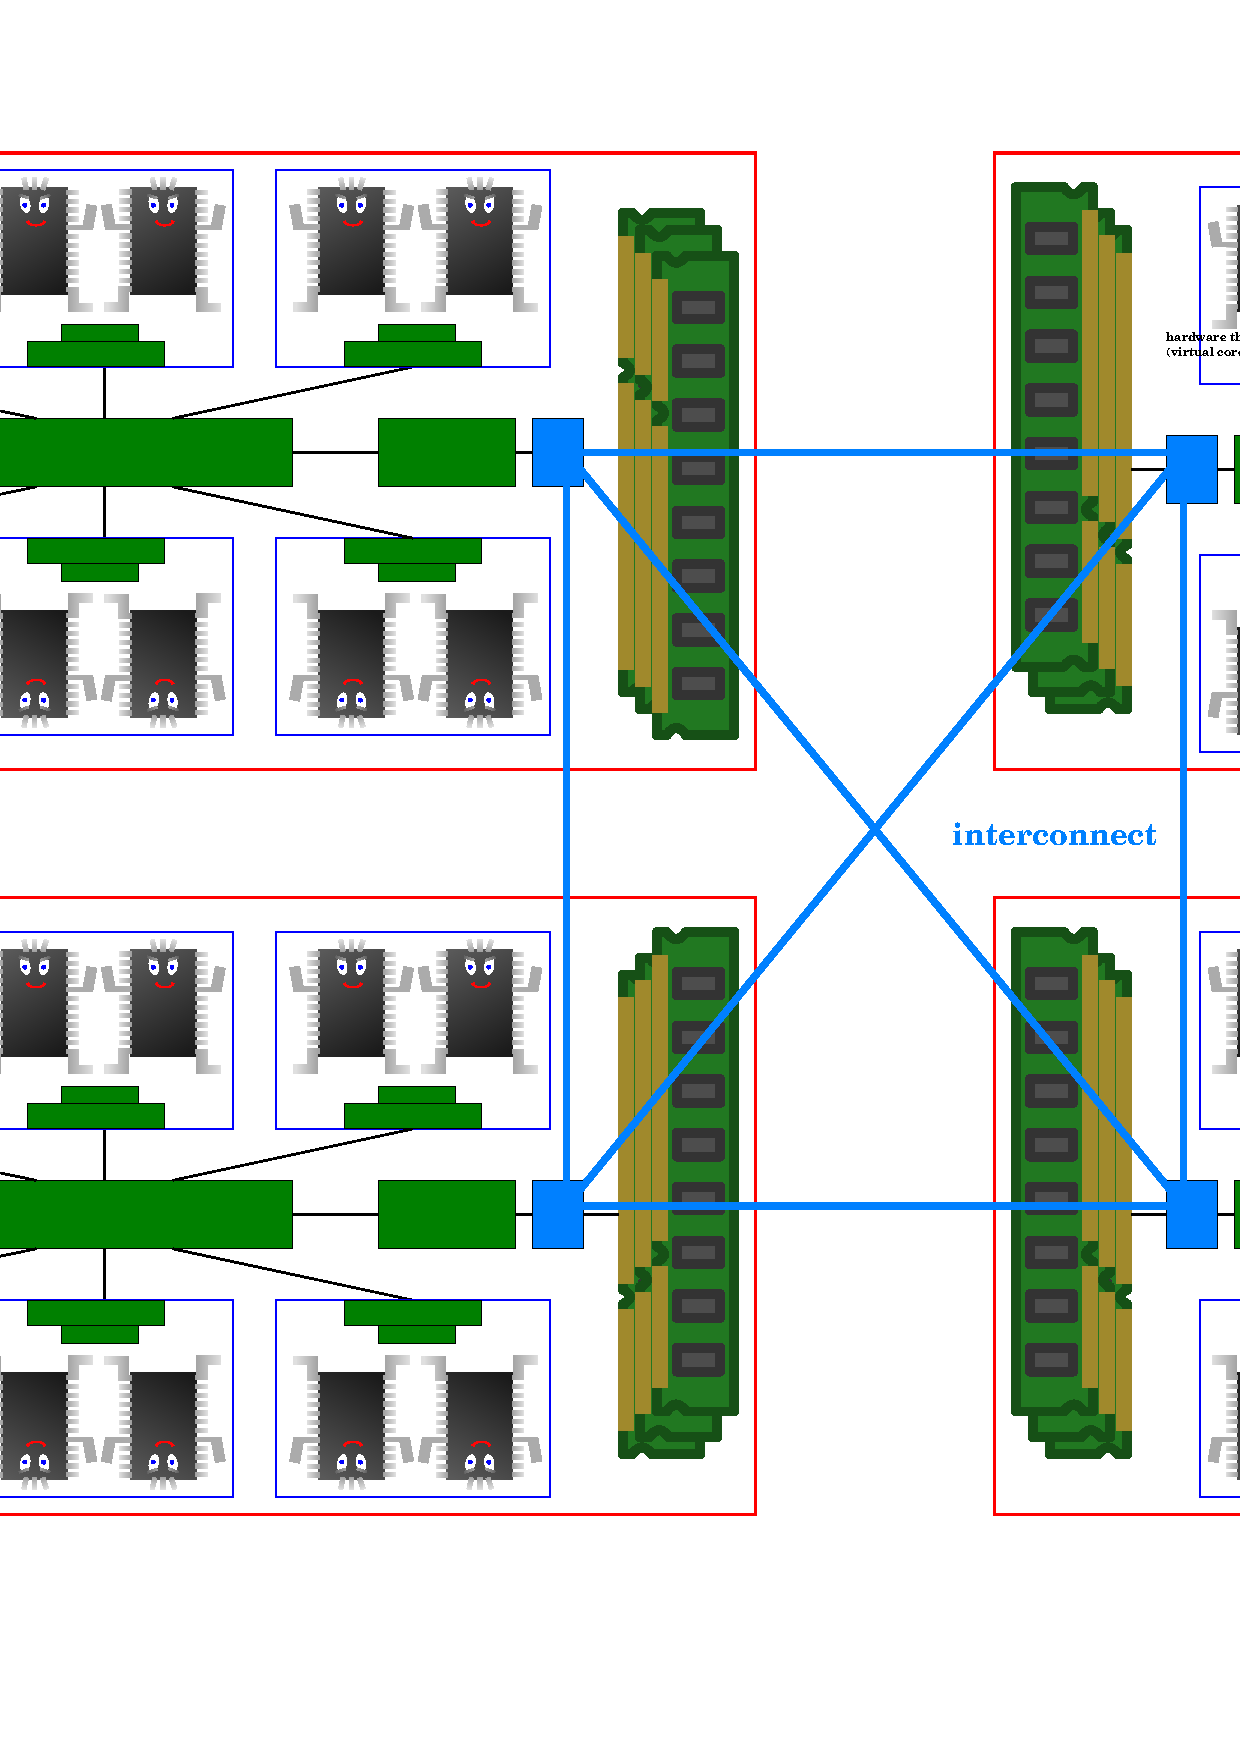
\includegraphics[width=0.40\textwidth]{out/pdf/svg/diagram_multisocket.pdf} \hspace{0.05\textwidth} \def\svgwidth{0.45\textwidth}\input{out/tex/svg/hierarchy.pdf_tex} %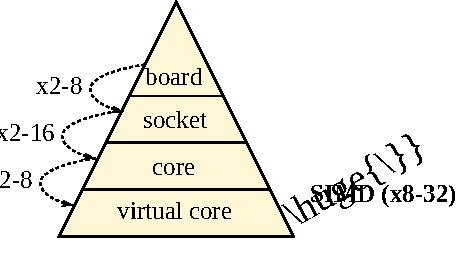
\includegraphics[width=0.4\textwidth]{out/pdf/svg/hierarchy.pdf}

\begin{itemize}
\item performance comes from \ao{\textit{multiplying}} parallelism of many levels
\item parallelism (per CPU)
\begin{center}
$=$ SIMD width $\times$ instructions/cycle $\times$ cores 
\end{center}
\item in particular, peak FLOPS (per CPU)
\begin{center}
$=$ (2 $\times$ SIMD width) $\times$ FMA insts/cycle/core $\times$ freq $\times$ cores
\end{center}
\item FMA: Fused Multiply Add ($d = a * b + c$)
\item the first factor of 2 : multiply and add (each counted as a flop)
\end{itemize}
\end{frame}

%%%%%%%%%%%%%%%%% 

\begin{frame}
\frametitle{What a GPU looks like?}
\begin{center}
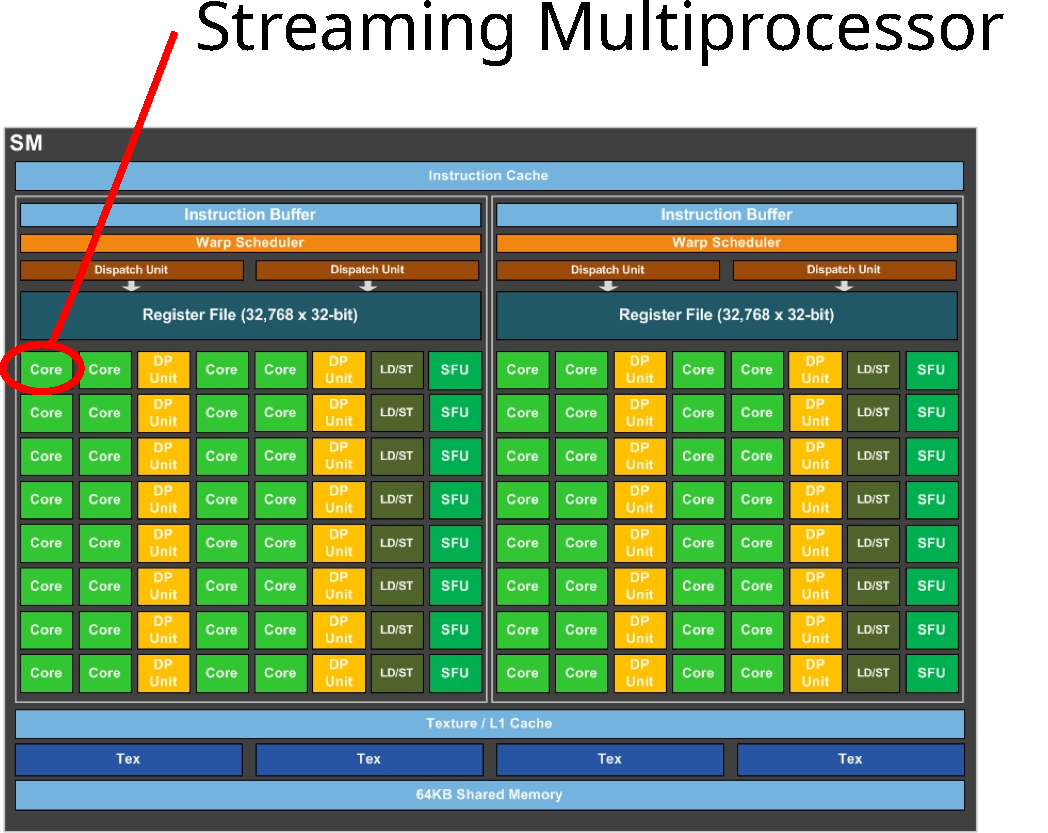
\includegraphics[width=0.5\textwidth]{out/pdf/svg/gpu.pdf}
\end{center}

\begin{itemize}
\item a GPU consists of many \ao{\it Streaming Multiprocessors (SM)}
\item each SM is highly multithreaded and can interleave many \ao{\it warps\/}
\item each warp consists of 32 \ao{\it CUDA threads}; in a single cycle,
  threads in a warp can execute the same single instruction
\end{itemize}

\end{frame}

%%%%%%%%%%%%%%%%% 
\begin{frame}
\frametitle{What a GPU looks like?}
\begin{itemize}
\item despite very different terminologies,
  there are more commonalities than differnces

\item []
  
  {\footnotesize
  \begin{tabular}{|c|c|}\hline
    GPU & CPU \\\hline
    SM & core \\
    multithreading in an SM & simultaneous multithreading \\
    a warp (32 CUDA threads) & a thread executing SIMD instructions \\
                & multiple instructions from a single thread \\\hline
  \end{tabular}}

\item there are significant differeces too, which we'll cover later
\end{itemize}

\end{frame}


%%%%%%%%%%%%%%%%% 
\begin{frame}
\frametitle{How much parallelism?}
\begin{itemize}
\item Intel CPUs

{\footnotesize
\begin{tabular}{|c|c|c|c|c|c|c|}\hline
arch       model             & SIMD & FMAs   & freq & core & peak      & TDP \\
                             & width& /cycle &      &      & GFLOPS    &     \\
                             & SP/DP& /core  & GHz  &      & SP/DP     & W   \\\hline
Haswell {\tiny E78880Lv3}    & 8/4  & 2      & 2.0  & 18   & 1152/576  & 115 \\
Broadwell {\tiny 2699v4}     & 8/4  & 2      & 2.2  & 22   & 1548/604  & 145 \\
Cascade Lake {\tiny 9282}    & 16/8 & 2  & 2.6  & 56   & 9318/4659 & 400 \\
\mura{Ice Lake {\tiny 8368}} & 16/8 & 2  & 2.4  & 38   & \mura{5836/2918} & 270 \\\hline
\end{tabular}}

\item NVIDIA GPUs (numbers are without Tensor Cores)

{\footnotesize
\begin{tabular}{|c|c|c|c|c|c|c|}\hline
acrh     model      & threads & FMAs   & freq  & SM       & paek   & TDP     \\
                    & /warp   & /cycle &       &          & GFLOPS &         \\
                    &         & /SM    &       &          &        &         \\
                    &         & SP/DP  & GHz   &          & SP/DP  & W       \\\hline
Pascal {\tiny P100} & 32  & 2/1 & 1.328 & 56  & 9519/4760  & 300     \\
Volta {\tiny V100}  & 32  & 2/1 & 1.530 & 80  & 15667/7833 & 300     \\
\mura{Ampere {\tiny A100}} & 32  & 2/1 & 1.410 & 108 & \mura{19353/9676} & 400     \\\hline
\end{tabular}}
\end{itemize}

\iffalse  
{\footnotesize
\begin{tabular}{|c|c|c|c|c|c|}\hline
acrh     model      & CUDA      & freq  & flops   & paek      & TDP     \\
                    & core      &       & /core   &           &         \\
                    &           & GHz   & /cycle  & GFLOPS    &         \\
                    &           & GHz   & SP/DP   & SP/DP     & W       \\\hline
Kepler {\tiny K80}  & 4992      & 0.560 & \ao{2/0.67}  & 5591/1864 & 300     \\
Maxwell {\tiny M60} & 4096      & 0.899 & \ao{2/0.063} & 7365/230  & 225-300 \\
Pascal {\tiny P100} & \mura{3584} & 1.328 & \ao{2/1}     & \aka{9519/4760} & 300     \\
Volta {\tiny V100} & \mura{5120} & 1.530 & \ao{2/1}     & \aka{15667/7833} & 300     \\\hline
\end{tabular}}
\fi

\end{frame}

%%%%%%%%%%%%%%%%%
\begin{frame}
\frametitle{Peak (SP) FLOPS}
\begin{columns}
  \begin{column}{0.5\textwidth}
  \begin{eqnarray*}
    &        & \mbox{Ice Lake 8368} \\
    & =      & (2 \times 16) \mbox{ [flops/FMA insn]} \\
    & \times & 2 \mbox{ [FMA insns/cycle/core]} \\
    & \times & 2.4\mbox{G [cycles/sec]} \\
    & \times & 38 \mbox{ [cores]} \\
    & = &      5836 \mbox{ GFLOPS}
  \end{eqnarray*}
  \end{column}
  \begin{column}{0.5\textwidth}
  \begin{eqnarray*}
    &        & \mbox{A100} \\
    & =      & (2 \times 32) \mbox{ [flops/FMA insn]} \\
    & \times & 2 \mbox{ [FMA insns/cycle/SM]} \\
    & \times & 1.41\mbox{G [cycles/sec]} \\
    & \times & 108 \mbox{ [SMs]} \\
    & = &      19353 \mbox{ GFLOPS}
  \end{eqnarray*}
  \end{column}
\end{columns}
\end{frame}

%%%%%%%%%%%%%%%%% 
\begin{frame}
\frametitle{NVIDIA: Tensor Cores}
\begin{itemize}
\item performance shown so far is limited by the fact that
  a single (FMA) instruction can perform 2 flops (1 multiply $+$ 1 add)
\item Tensor Core, a special execution unit for a small matrix-multiply-add, changes that
\item \href{https://images.nvidia.com/aem-dam/en-zz/Solutions/data-center/nvidia-ampere-architecture-whitepaper.pdf}{A100's each Tensor Core} can do $C = A \times B + C$ (where $A : 4\times 4$, $B : 4 \times 8$)
  per cycle ($A : 4 \times 4$ TF32, $B : 4 \times 8$ TF32, $C$ and $D$ are SP)
  \[ 2 \times 4 \times 4 \times 8 = 256 \mbox{ flops/cycle} \]
\item each SM of A100 GPU has 4 Tensor Cores, so a single A100 device can do
  \begin{eqnarray*}
    &        & (2 \times 4 \times 4 \times 8) \mbox{ [flops/cycle]} \\
    & \times & 1.41\mbox{G [cycles/sec]} \\
    & \times & 4 \times 108 \mbox{ [Tensor Cores]} \\
    & = &      \href{https://www.nvidia.com/content/dam/en-zz/Solutions/Data-Center/a100/pdf/nvidia-a100-datasheet-nvidia-us-2188504-web.pdf}{155934.72} \mbox{ GFLOPS}
  \end{eqnarray*}
\end{itemize}
\end{frame}

\iffalse
%%%%%%%%%%%%%%%%% 
\begin{frame}
\frametitle{Intel: VNNI}
\begin{itemize}
\item Intel Cascade Lake and Ice Lake have similar special instructions
  for 16 bit and 8 bit integers
\end{itemize}
\end{frame}
\fi

\iffalse
%%%%%%%%%%%%%%%%% 
\begin{frame}
\frametitle{Tensor Cores}
\begin{itemize}
\item performance shown so far is limited by the fact that
  a single (FMA) instruction can perform 2 flops (1 multiply $+$ 1 add)
\item Tensor Core, a special execution unit for a small matrix-multiply-add, changes that
\item V100's each Tensor Core can  $C = A \times B + C$ for $4\times 4$ matrices
  \[ 2 \times 4 \times 4 \times 4 = 128 \mbox{ flops} \]
  per cycle ($A$ and $B$ are HP (Half Precision; 16 bit) and $C$ and $D$ are either HP or SP)
\item V100 GPU has 640 Tensor Cores
  \begin{eqnarray*}
    &        & \mbox{Volta V100} \\
    & =      & (2 \times 4 \times 4 \times 4) \mbox{ [flops/MMA insn]} \\
    & \times & 1.53\mbox{G [cycles/sec]} \\
    & \times & 640 \mbox{ [Tensor Cores]} \\
    & = &      125337.6 \mbox{ GFLOPS}
  \end{eqnarray*}
\item more recent models, A100, has Tensor Cores on other data types
\end{itemize}
\end{frame}
\fi

\iffalse
\begin{frame}
\frametitle{How much parallelism?}
\begin{itemize}
\item don't be spoofed by terminologies
  \begin{itemize}
  \item a single CUDA core is not anything similar to a single CPU core
  \item a single CUDA core $\approx$ a single SIMD lane
  \item frequency and throughputs per cycle also count
  \item after all it's performance (or performance/watt) that counts, not
    parallelism
  \end{itemize}
\item even peak performance (let alone parallelism) may not be a meaningful proxy of 
  performance in real apps
\end{itemize}
\end{frame}
\fi

%%%%%%%%%%%%%%%%%
\begin{frame}
\frametitle{Trends}
\begin{itemize}
\item processors' performance improvement is getting less and less ``generic'' or ``transparent''
  \begin{itemize}
  \item frequencey $+$ instruction level parallelism
  \item [] $\rightarrow$ explicit parallelism (multicore/manycore)
  \item [] $\rightarrow$ special execution unit for macro operations (e.g., MMA)
  \item [] $\rightarrow$ application-specific instructions (?)
  \end{itemize}
\item performance is getting more and more dependent on programming 
\end{itemize}
\end{frame}

%=================================
\section{How to Program Parallel Machines?}
%=================================

%%%%%%%%%%%%%%%%% 
\begin{frame}
\frametitle{So how to program it?}

\begin{itemize}
\item no matter how you program it, you want to maximally utilize 
  all forms of parallelism
\item ``how'' depends on devices and programming languages 
\end{itemize}
\end{frame}

%%%%%%%%%%%%%%%%% 
\begin{frame}
\frametitle{Language constructs for multiple cores / GPUs}
from low level to high levels
\begin{itemize}
\item (CPU) OS-level threads 
\item (GPU) CUDA threads
\item \ao{SPMD} $\approx$ the entire program runs with $N$ threads
\item \ao{parallel loops}
\item dynamically created \ao{tasks}
\item internally parallelized \ao{libraries} (e.g., matrix operations)
\item high-level languages executing pre-determined operations 
  (e.g., matrix operations, \ao{map \& reduce}-like patterns, deep learning) in parallel
\end{itemize}
\end{frame}

%%%%%%%%%%%%%%%%% 
\begin{frame}
\frametitle{Language constructs for CPU SIMD}
from low level to high levels
\begin{itemize}
\item assembly
\item intrinsics
\item vector types
\item vectorized loops
\item internally vectorized libraries (e.g., matrix operations)
\end{itemize}
\end{frame}

%%%%%%%%%%%%%%%%% 
\begin{frame}
\frametitle{This lecture is for \ldots}
those who want to:
\begin{itemize}
\item<1-> have a first-hand experience in parallel and high performance programming
  \ao{(OpenMP, CUDA, SIMD, \ldots)}
\item<2-> know good tools to solve more complex problems in parallel
  \ao{(divide-and-conquer and task parallelism)}
\item<3-> understand when you can get ``close-to-peak'' CPU/GPU performance and how to get it
  \ao{(SIMD and instruction level parallelism)}
\item<4-> learn many reasons why you don't get good parallel performance
\item<5-> have a good understanding about \ao{caches} and \ao{memory}
  and why they matter so much for performance
\end{itemize}
\end{frame}

\end{document}
